% This file was created with matplot2tikz v0.4.0.
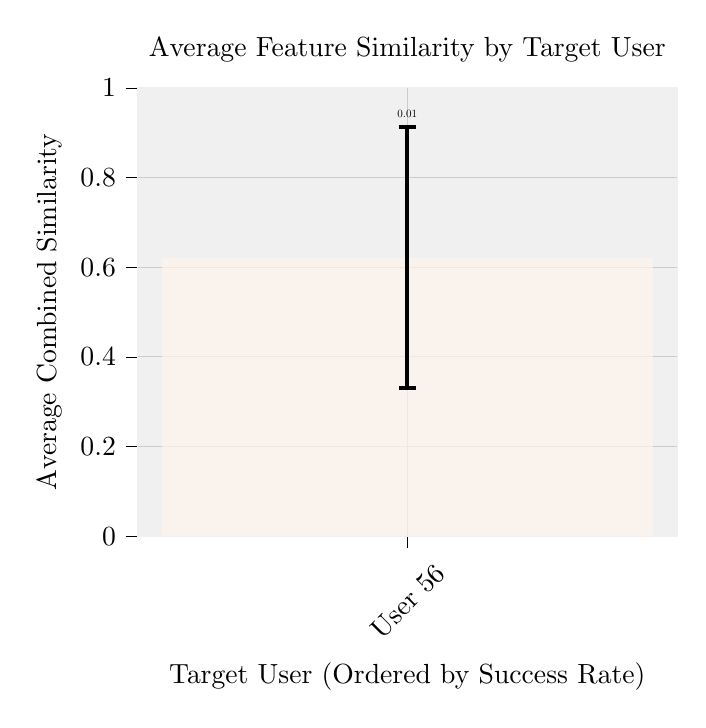
\begin{tikzpicture}

\definecolor{lightgray203}{RGB}{203,203,203}
\definecolor{seashell254243237}{RGB}{254,243,237}
\definecolor{whitesmoke240}{RGB}{240,240,240}

\begin{axis}[
axis background/.style={fill=whitesmoke240},
axis line style={whitesmoke240},
tick align=outside,
tick pos=left,
title={Average Feature Similarity by Target User},
x grid style={lightgray203},
xlabel={Target User (Ordered by Success Rate)},
xmajorgrids,
xmin=-0.44, xmax=0.44,
xtick style={color=black},
xtick={0},
xticklabel style={rotate=45.0},
xticklabels={User 56},
y grid style={lightgray203},
ylabel={Average Combined Similarity},
ymajorgrids,
ymin=0, ymax=1,
ytick style={color=black}
]
\draw[draw=none,fill=seashell254243237,fill opacity=0.7,very thin] (axis cs:-0.4,0) rectangle (axis cs:0.4,0.621539116876937);
\path [draw=black, ultra thick]
(axis cs:0,0.329921103706325)
--(axis cs:0,0.91315713004755);

\addplot [ultra thick, black, mark=-, mark size=3, mark options={solid}, only marks]
table {%
0 0.329921103706325
};
\addplot [ultra thick, black, mark=-, mark size=3, mark options={solid}, only marks]
table {%
0 0.91315713004755
};
\draw (axis cs:0,0.93315713004755) node[
  scale=0.4,
  anchor=base,
  text=black,
  rotate=0.0
]{0.01};
\end{axis}

\end{tikzpicture}
